\documentclass[11pt,letterpaper]{article}
\usepackage{macroshw}

\title{\begin{spacing}{1.2}Quantum Mechanics I\\HW 3\end{spacing}}
\author{Matthew Phelps}
\date{Due: March 5}

\begin{document}
\maketitle

% #1
\begin{enumerate}
  \item 
  
  
  A quantum particle is confined to the interval $[-a,a]$. It is described by the time dependent wave function
  \[
  	\psi(x,t) = \frac{1}{\sqrt{2a}}\left\{\cos\left(\frac{\pi}{2a}x\right)\exp{\left[-i\left(\frac{\hbar\pi^2}{8ma^2}t\right)		\right]}-\sin\left(\frac{\pi}{a}x\right)\exp{\left[-i\left(\frac{\hbar\pi^2}{2ma^2}t\right)\right]}\right\}
  \]
  
    \begin{enumerate}
    % 		1(a)
\item Show that $\psi(x,t)$ is properly normalized and find the associated probability current $J(x,t)$.
\\
\\
Before we normalize we rewrite our wavefunction as
\begin{equation}\label{1}\psi = \frac{1}{\sqrt{2a}}[\cos(sx)\exp{(-iut)}-\sin(2sx)\exp{(-i4ut)}]\end{equation}
and so
\begin{equation}\label{2}\psi^* = \frac{1}{\sqrt{2a}}[\cos(sx)\exp{(iut)}-\sin(2sx)\exp{(i4ut)}]\end{equation}
thus
\begin{align*}|\psi|^2 = \frac{1}{2a}&[\cos^2(sx)+\sin^2(2sx)-\cos(sx)\sin(2sx)\exp(-iut)\exp(i4ut)]\\
&-\cos(sx)\sin(2sx)\exp(-i4ut)\exp(iut)].
\end{align*}
Note that
$$\exp(-iut)\exp(i4ut)+\exp(-i4ut)\exp(iut) = \exp(i3ut)+\exp(-i3ut) = 2\cos(3ut)$$
so we then have
\begin{equation}\label{4} |\psi|^2 = \frac{1}{2a}[\cos^2(sx)+\sin^2(2sx)-2\cos(sx)\sin(2sx)\cos(3ut)].\end{equation}
Normalizing,
$$\frac{1}{2a}\int_{-a}^a{dx\ [\cos^2(sx)+\sin^2(2sx)-2\cos(sx)\sin(2sx)\cos(3ut)]}. $$
Since the last term is odd and the first two are even we then have
$$\frac{1}{a}\int_{0}^a{dx\ [\cos^2(sx)+\sin^2(2sx)]}. $$
Using the half angle formulas
\begin{align*}&\quad\frac{1}{a}\int_{0}^a{dx\ \left[\frac{1+\cos(2sx)}{2}+\frac{1-\cos(4sx)}{2}\right]}\\
&=\frac{1}{a}\left.\left[x+\frac{1}{4s}\sin(2sx)-\frac{1}{8s}\sin(4sx)\right]\right|_0^a\\
&=\frac{1}{a}\left.\left[x+\frac{1}{4s}\sin(2sx)-\frac{1}{8s}\sin(4sx)\right]\right|_a\\
&=\frac{1}{a}\left.\left[x+\frac{a}{2\pi}\sin\left(\frac{\pi}{a}x\right)-\frac{a}{4\pi}\sin\left(\frac{2\pi}{a}x\right)\right]\right|_a\\
&=\frac{1}{a}(a)\\
&=1.
\end{align*}
Therefore
$$\int_{-a}^a{dx\ |\psi(x,t)|^2} = 1.$$
There are a few ways one could compute the probability current (Sakurai p.100-101). One particular method is to use
\begin{equation}\label{3}\vect j = \frac{\hbar}{m}\Im(\psi^*\nabla\psi).\end{equation}
Another method involves expressing the wavefunction in polar form, however, this turned out to give a much too cumbersome equation when I attempted it. For our one dimensional wavefunction \eqref 1 we have
$$\frac{\partial\psi}{\partial x} = \frac{1}{\sqrt{2a}}[-s\sin(sx)e^{-iut}-2s\cos(2sx)e^{-i4ut}]$$
and from \eqref 2 we have
$$\psi^* = \frac{1}{\sqrt{2a}}[\cos(sx)e^{iut}-\sin(2sx)e^{i4ut}].$$
Multiplying
\begin{align*}\psi^*\nabla\psi = &\frac{1}{2a}[-s\sin(sx)\cos(sx)+2s\sin(2sx)\cos(2sx) \\
&\ +s\sin(sx)\sin(2sx)e^{i3ut}-2s\cos(sx)\cos(2sx)e^{-i3ut}].
\end{align*}
Since we are looking for the imaginary part, the only terms that remain are 
\begin{align*}\Im{(\psi^*\nabla\psi)}&= \frac{1}{2a}[s\sin(sx)\sin(2sx)\sin(3ut)+2s\cos(sx)\cos(2sx)\sin(3ut)]\\
&=\frac{1}{2a}\{2s\cos(sx)\sin(3ut)[\sin^2(sx)+\cos(2sx)]\}\\
&=\frac{1}{2a}\{2s\cos(sx)\sin(3ut)[\sin^2(sx)+\cos^2(sx)-\sin^2(sx)]\}\\
&=\frac{1}{2a}[2s\cos^3(sx)\sin(3ut)]\\
&=\frac{1}{2a}\left[\frac{\pi}{a}\cos^3\left(\frac{\pi}{2a}x\right)\sin\left(\frac{3\hbar\pi^2}{8ma^2}t\right)\right].
\end{align*}
Using \eqref 3 the probability flux $\vect j=j(x,t)\vecth x$ is then expressed as
\begin{equation}\label{6}j(x,t) = \frac{\hbar}{2ma}\left[\frac{\pi}{a}\cos^3\left(\frac{\pi}{2a}x\right)\sin\left(\frac{3\hbar\pi^2}{8ma^2}t\right)\right].\end{equation}

% 	1(b)
\item Compute the probability
  $$P_{left} = \int_{-a}^0{dx|\psi(x,t)|^2}$$
  for finding the particle in the left half of the interval.
  \\ \\Using \eqref 4 we have
  $$ |\psi|^2 = \frac{1}{2a}[\cos^2(sx)+\sin^2(2sx)-2\cos(sx)\sin(2sx)\cos(3ut)]$$
  and so
  $$\int_{-a}^0{dx\ |\psi|^2 } = \frac{1}{2a}\int_{-a}^0{dx\ [\cos^2(sx)+\sin^2(2sx)-2\cos(sx)\sin(2sx)\cos(3ut)]}.$$
  This integral is almost the same as when we did the normalization, so we will be able to save work and use that result. Using the earlier result of
  $$\frac{1}{a}\int_{0}^a{dx\ [\cos^2(sx)+\sin^2(2sx)]}  =\frac{1}{a}\left.\left[x+\frac{a}{2\pi}\sin\left(\frac{\pi}{a}x\right)-\frac{a}{4\pi}\sin\left(\frac{2\pi}{a}x\right)\right]\right|_0^a$$
  we see that
  \begin{align*}\frac{1}{2a}\int_{-a}^0{dx\ [\cos^2(sx)+\sin^2(sx)]} &= \frac{1}{2a}\left.\left[x+\frac{a}{2\pi}\sin\left(\frac{\pi}{a}x\right)-\frac{a}{4\pi}\sin\left(\frac{2\pi}{a}x\right)\right]\right|_{-a}^0\\
&=  \frac{-1}{2a}\left.\left[x+\frac{a}{2\pi}\sin\left(\frac{\pi}{a}x\right)-\frac{a}{4\pi}\sin\left(\frac{2\pi}{a}x\right)\right]\right|_{-a}\\
&=  \frac{-1}{2a}\left[-a+\frac{a}{2\pi}\sin\left(-\pi\right)-\frac{a}{4\pi}\sin\left(-2\pi\right)\right]\\
&=\frac{1}{2}.
  \end{align*}
  We are now left with the integration of
  \begin{align*}\frac{-\cos(3ut)}{a}\int_{-a}^0{dx\ [\cos(sx)\sin(2sx)]} &= \frac{-\cos(3ut)}{a}\int_{-a}^0{dx\ [\cos(sx)\sin(2sx)]} \\
  &=\frac{-2\cos(3ut)}{a}\int_{-a}^0{dx\ [\cos^2(sx)\sin(sx)]}\\
  &=\frac{-2\cos(3ut)}{a}\left.\left[\frac{\cos^3(sx)}{-3s}\right]\right|_{-a}^0\\
  &=\frac{2\cos(3ut)}{3a}\left(\frac{1}{s}-\frac{\cos^3(-as)}{s}\right)\\
  &=\frac{2\cos(3ut)}{3a}\left(\frac{2a}{\pi}-\frac{2a\cos^3\left(-\frac{\pi}{2}\right)}{\pi}\right)\\
  &=\frac{4}{3\pi}\cos\left(\frac{3\hbar\pi^2}{8ma^2}t\right).
  \end{align*}
  Therefore we have
  \begin{equation}\label{5}P_{left} = \frac{1}{2}+\frac{4}{3\pi}\cos\left(\frac{3\hbar\pi^2}{8ma^2}t\right).\end{equation}
% 	1(c)
\item Compare the probabilities $P_{left}(0)$ and $P_{left}(\tau)$ where $\tau = \frac{4ma^2}{\hbar\pi}$ and show that $P_{left}(0)>P_{left}(\tau)$.
\\ \\Using \eqref 5 we see that
$$P_{left}(0) = \frac{1}{2}+\frac{4}{3\pi}$$
$$P_{left}(\tau) = \frac{1}{2}+\frac{4}{3\pi}\cos\left(\frac{3\pi}{2}\right) = \frac{1}{2}.$$
Therefore
$$P_{left}(0)>P_{left}(\tau).$$\\
% 	1(d)
\item Show that $P_{left}(0)-P_{left}(\tau) = \int_0^\tau{dt\ J(0,t)}$ and interpret the result. 
 \\ \\First note that from \eqref 6 
 $$ j(0,t) = \frac{\hbar\pi}{2ma^2}\sin\left(\frac{3\hbar\pi^2}{8ma^2}t\right) $$
 and so
 \begin{align*}\int_0^\tau{dt\ j(0,t)} &= \frac{\hbar\pi}{2ma^2}\int_0^\tau{dt\ \sin\left(\frac{3\hbar\pi^2}{8ma^2}t\right)}\\
 &= \frac{\hbar\pi}{2ma^2}\left.\left[-\frac{8ma^2}{3\hbar\pi^2}\cos\left(\frac{3\hbar\pi^2}{8ma^2}t\right)\right]\right|_0^\tau\\
 &= \frac{\hbar\pi}{2ma^2}\left(\frac{8ma^2}{3\hbar\pi^2}\right)\\
 &=\frac{4}{3\pi}
 \end{align*}
 and thus
  $$P_{left}(0)-P_{left}(\tau) = \int_0^\tau{dt\ j(0,t)}\ \to\ \left(\frac{4}{3\pi}+\frac{1}{2}\right)-\frac{1}{2}=\frac{4}{3\pi}.$$
  The idea is that the flow of probability flux through a surface at the origin (or a point in this case) integrated over time $t=0 \to t=\tau$ is equal to the total change in probability at times $t=0$ and $t=\tau$. Since the total probability is conserved, the change in probability on the left half of the ``box" would have to manifest itself as a flux past a particular point. If you like, it is a realization of the continuity equation. See \href{http://physics.stackexchange.com/questions/145048/do-the-probability-density-and-the-probability-current-density-have-a-unit}{here} for a good discussion on units and how to picture it.
  \end{enumerate}
% #2
\item Sakurai 2.22: Consider a particle of mass $m$ subject to a one-dimensional potential of the following form:
$$V=\begin{cases}\frac{1}{2}kx^2&\quad\text{for}\ x>0\\\infty&\quad\text{for}\ x<0\end{cases}$$
\begin{enumerate}
% 	2(a)
\item What is the ground-state energy?
\\ \\This is that of a half harmonic oscillator if you like. Since the harmonic oscillator is an even function, it has solutions that are both even and odd. Looking at the first couple states
$$\braket{x'|0} = \left(\frac{1}{\pi^{1/4}\sqrt{x_0}}\right)\exp{\left[-\frac{1}{2}\left(\frac{x'}{x_0}\right)^2\right]}$$
$$\braket{x'|1} = \left(\frac{1}{\sqrt 2x_0}\right)\left(x'-x_0^2\frac{d}{dx'}\right)\braket{x'|0}$$
we can see that the ground state is even and subsequent analysis easily shows that all odd-numbered states are odd states. However, for the half harmonic oscillator we must be careful to note that our normalization changes. Specifically,
$$A^2\int_{-\infty}^{\infty}{dx\ |\psi_1(x)|^2} = 2A^2\int_{0}^{\infty}{dx\ |\psi_1(x)|^2}=1$$
$$A = \left[\frac{1}{2}\frac{1}{\int_{0}^{\infty}{dx\ |\psi_1(x)|^2}}\right]^{1/2}$$
where we have used the fact that $|\psi|^2$ is even for an odd (real) state. 
For the half-harmonic oscillator, the factor of $2$ goes away and so the relation between normalizations is
$$A = \frac{1}{\sqrt2}A_H.$$
Despite this difference, the eigenvalues of the energies do not change based on the normalization and  the ground state energy for the half harmonic oscillator is the same as that for the state $\braket{x'|1}$
which corresponds to an energy of 
$$E = \frac{3}{2}\h\omega.$$


% 	2(b)
\item What is the expectation value of $\braket{x^2}$ for the ground state?
\\ \\There are three methods to solve this problem. The first, most obvious, and most painful would be to do the full integration. The second method is to express $x^2$ in terms of raising and lowering operators, in which orthogonal states cancel and we are left with the coefficients produced from the raising/lowering operator. A solid method for sure (probably the best). The last method, which we will use, will be the Virial theorem which states
$$\braket{T} = \frac{1}{2}\braket{x\frac{dV}{dx}}.$$
For the harmonic oscillator,
$$\frac{dV}{dx} = m\omega^2x$$
$$x\frac{dV}{dx} = m\omega^2x^2.$$
Therefore
$$\braket{T} = \braket{V}.$$
Using the raising and lowering operators (see we still needed them!) or integration, we can find that for the $n$th state of the harmonic oscillator 
$$\braket{T} = \frac{1}{2}\left(n+\frac{1}{2}\right)\hbar\omega.$$
Now we can use
\begin{align*}\braket{x^2} &= \frac{2}{m\omega^2}\braket{V}\\
&=\frac{2}{m\omega^2}\braket{T}\\
&=\frac{\h}{m\omega}\left(n+\frac{1}{2}\right).
\end{align*}
Thus for our $n=1$ state, we have
$$\braket{x^2} = \frac{3\hbar}{2m\omega}.$$
We cannot forget the normalization difference here, however. We will simply need to multiply by $(\sqrt2)^2$ to finally arrive at
$$\braket{x^2} = \frac{3\hbar}{m\omega}.$$
\end{enumerate}
% #3
\item Sakurai 2.24: Consider a particle in dimension bound to a fixed center by a $\delta$-function potential of the form
$$V(x) = -\nu_0\delta(x),\quad(\nu_0\in\mathbb{R}\cap\nu_0>0)$$
Find the wavefunction and the binding energy of the ground state. Are there excited bound states?
\\ \\First note that if $E>0$ we will have scattering states while $E<0$ will give us bound states. Therefore we will be looking for solutions for $E<0$. Our task here basically amounts to solving the Schrodinger equation for all regions of interest, and connecting them all together. Our wavefunction will be everywhere continuous, but we can expect a discontinuity in the derivative at the origin. 
\\ \\Starting with the region $x<0$, our potential here is zero and so the TISE reads
$$-\frac{\h^2}{2m}\frac{d^2\psi}{dx^2} = E\psi$$
$$\frac{d^2\psi}{dx^2} = -\frac{2mE}{\h^2}\psi = -k^2\psi$$
with familiar solutions of
$$\psi_-(x) = Ae^{-ikx}+Be^{ikx}$$
where $$k\equiv\frac{\sqrt{2mE}}{\h}=\frac{i\sqrt{2m|E|}}{\h}.$$
Since $E<0$, we get an $i$ from the $k$ and the exponentials are in fact the normal non-oscillatory exponentials. As such, in the limit $x\to\-\infty$ we must have a normalizable wavefunction and thus
$$B= 0$$
$$\psi_-(x) = Ae^{-ikx}.$$
Similarly for $x>0$ we again have the same solution to the Schrodinger equation, that is
$$\psi_+(x) = Ce^{-ikx}+De^{ikx}$$
where $k$ remains the same. This time as $x\to\infty$ it is instead 
$$C=0$$
$$\psi_+(x) = De^{ikx}$$
Imposing our first boundary condition of continuity at the origin we see that 
$$\psi_-(0) = \psi_+(0)$$
so
$$A=D.$$
Now we have
$$\psi(x) = \begin{cases}Ae^{-ikx}&\quad\text{for}\quad x\le 0\\Ae^{ikx}&\quad\text{for}\quad x\ge 0\end{cases}.$$
To find $A$ or $k$, we must find determine the magnitude of the discontinuity in the derivative. To achieve this, what we shall do is integrate the Schrodinger equation across the origin and take the limit:
$$\lim_{\epsilon\to 0}\left[ -\frac{\h^2}{2m}\int_{-\epsilon}^{+\epsilon}{dx\ \frac{d^2\psi}{dx^2}}+\int_{-\epsilon}^{+\epsilon}{dx\ V(x)\psi(x)}\right] = \lim_{\epsilon\to 0}\left[E\int_{-\epsilon}^{+\epsilon}{dx\ \psi(x)}\right] 
$$
$$\lim_{\epsilon\to 0}\left[\left.\frac{d\psi_+}{dx}\right|_{+\epsilon}-\left.\frac{d\psi_-}{dx}\right|_{-\epsilon}\right] = \frac{2m}{\h^2}\lim_{\epsilon\to 0}\int_{-\epsilon}^{+\epsilon}{dx\ -\nu_0\delta(x)\psi(x)}
$$
where we note that any finite integrand will vanish in the limit that the bounds approach zero. This would be the reason why the derivative of $\psi$ is ordinarily continuous; $\Delta\left(\frac{d\psi}{dx}\right) \to 0$. But here we have the delta function that prevents this:
$$\Delta\left(\frac{d\psi}{dx}\right)= \frac{2m}{\h^2}\lim_{\epsilon\to 0}\int_{-\epsilon}^{+\epsilon}{dx\ -\nu_0\delta(x)\psi(x)}
$$
$$\Delta\left(\frac{d\psi}{dx}\right)= -\frac{2m\nu_0}{\h^2}\psi(0).$$
This tells us the discontinuity in the derivative. What we must do now is equate it to our wavefunction derivatives:
$$\left.\frac{d\psi_+}{dx}\right.|_0 = ikA$$
$$\left.\frac{d\psi_-}{dx}\right.|_0 = -ikA$$
$$\Delta\left(\frac{d\psi}{dx}\right) = 2ikA $$
which tells us that
$$2ikA= -\frac{2m\nu_0}{\h^2}\psi(0)$$
$$2ikA= -\frac{2m\nu_0}{\h^2}A$$
$$k = i\frac{m\nu_0}{\h^2}$$
$$\frac{\sqrt{2mE}}{\h}=i\frac{m\nu_0}{\h^2}$$
$$E = -\frac{m\nu_0^2}{2\h^2}.$$
This is the energy of our single bound state - no excited bound states are present. To find the wavefunction, we normalize $A$. Using 
$$\psi(x) = \begin{cases}A\exp{\left(\frac{m\nu_0}{\h^2}x\right)}&\quad\text{for}\quad x\le 0\\ A\exp{\left(-\frac{m\nu_0}{\h^2}x\right)}&\quad\text{for}\quad x\ge 0\end{cases}$$
we then have 
\begin{align*}A^2\int_{-\infty}^{\infty}{dx\ |\psi(x)^2}| &= A^2\int_{-\infty}^0{dx\ \exp{\left(\frac{2m\nu_0}{\h^2}x\right)}}+A^2\int^{\infty}_0{dx\ \exp{\left(\frac{-2m\nu_0}{\h^2}x\right)}}\\
&=2A^2\int^{\infty}_0{dx\ \exp{\left(\frac{-2m\nu_0}{\h^2}x\right)}}\\
&=2A^2\left.\left[-\frac{\h^2}{2m\nu_0} \exp{\left(\frac{-2m\nu_0}{\h^2}x\right)}\right]\right|_0^{\infty}\\
1&=2A^2\frac{\h^2}{2m\nu_0}\\
A&=\frac{\sqrt{m\nu_0}}{\h}.
\end{align*}
Therefore our wavefunction and energy are:
$$\psi(x) = \frac{\sqrt{m\nu_0}}{\h}\exp{\left(-\frac{m\nu_0|x|}{\h^2}\right)};\quad E = -\frac{m\nu_0^2}{2\h^2}. $$
% #4
\item Sakurai 2.28: Consider an electron confined to the \emph{interior} of a hollow cylindrical shell whose axis coincides with the $z$-axis. The wave function is required to vanish on the inner and outer walls, $\rho = \rho_a$ and $\rho_b$, and also at the top and bottom, $z=0$ and $L$. 
\begin{enumerate}
% 	4(a)
\item Find the energy eigenfunctions. (Do not bother with normalization.) Show that the energy eigenvalues are given by 
$$E_{lmn} = \left(\frac{\h^2}{2m_e}\right)\left[k^2_{mn}+\left(\frac{l\pi}{L}\right)^2\right]\quad(l=1,2,3,..\ m=0,1,2,..)$$
where $k_{mn}$ is the $n$th root of the transcendental equation
$$J_m(k_{mn}\rho_b)N_m(k_{mn}\rho_a)-N_m(k_{mn}\rho_b)J_m(k_{mn}\rho_a)=0.$$
\\ In this problem, we have no potential and thus the TISE will have the form
$$-\frac{\h^2}{2m}\del^2\psi -E\psi = 0$$
which can easily be cast into the form of the Helmholtz equation, namely
$$\del^2\psi +j^2\psi = 0$$
where 
$$j\equiv \sqrt{\frac{2mE}{\h^2}}.$$
Our task amounts to solving the TISE for the specified boundary conditions. To solve this particular PDE (cf. Arfken p. 421) we first write it down in cylindrical coordinates:
$$\frac 1\rho \frac{\partial}{\partial \rho}\left(\rho\frac{\partial \psi}{\partial\rho}\right)+\frac{1}{\rho^2}\frac{\partial^2\psi}{\partial\phi^2}+\frac{\partial^2\psi}{\partial z^2}+j^2\psi = 0.$$
Observing that our differential operators are all additive, we try separation of variables,
$$\psi(\rho,\phi,z) = P(\rho)\Phi(\phi)Z(z).$$
Substituting this in, we have
$$\frac {\Phi Z}{\rho} \frac{d}{d \rho}\left(\rho\frac{dP}{d\rho}\right)+\frac{PZ}{\rho^2}\frac{d^2\Phi}{d\phi^2}+P\Phi\frac{d^2Z}{dz^2}+j^2P\Phi Z = 0$$
$$\frac{1}{\rho P}\frac{d}{d\rho}\left(\rho\frac{dP}{d\rho}\right)+\frac{1}{\rho^2\Phi}\frac{d^2\Phi}{d\phi^2}+j^2 = -\frac{1}{Z}\frac{d^2Z}{dz^2}.$$
Since we have isolated some function $f(z)$ on the RHS, we choose to set it equal to $h^2$. I don't like the choices of separation variables here, but to conform to the final answer given in the text we will have to use some non-customary ones. The decision to choose $h^2$ to be positive requires some foresight on our boundary conditions. First observe that 
$$\frac{d^2Z}{dz^2} = \pm h^2Z.$$
A positive coeffecient leads to a hyperbolic function while a negative leads to an oscillating exponential. Since the B.C.'s require $Z(z)$ to vanish at \emph{two} faces of the cylinder, we can certainly rule out the hyperbolic functions. Hence the choice of $h^2$ on the RHS of the D.E. As such we now have
$$Z(z)\propto e^{\pm ihz}.$$
If we now denote a new constant 
$$k^2\equiv j^2-h^2$$
we can reform our equation as
$$\frac{\rho}{P}\frac{d}{d\rho}\left(\rho\frac{dP}{d\rho}\right)+k^2\rho^2 = -\frac{1}{\Phi}\frac{d^2\Phi}{d\phi^2}.$$
Lets use the separation constant $m^2$ for this one, in which we have
$$\frac{d^2\Phi}{d\phi^2} = -m^2\Phi;\quad\Phi(\phi)\propto e^{\pm im\phi}.$$
In using $\phi$ as the azimuthal angle, we impose the B.C. of periodicity and find that $m$ must be an integer:
$$\Phi(\phi) = \Phi(\phi+2\pi)\rightarrow e^{\pm im\phi}=e^{\pm i(m+2\pi)\phi} = e^{\pm im\phi}+e^{\pm im2\pi}.$$
For the $\rho$ dependence we are left with 
\begin{equation}\label{bde}\rho\frac{d}{d\rho}\left(\rho\frac{dP}{d\rho}\right)+(k^2\rho^2-m^2)P = 0.
\end{equation}
If we use a change of variable $x\equiv k\rho,$ this becomes Bessel's differential equation! The solutions to this equation are of course the Bessel functions of order $m$. The Bessel functions of the first, second, and third kind are denoted $J_m(x)$, $N_m(x)$, and $H_m(x)$ respectively. The last two are at times referred to as the Neumann and Hankel functions. The solution to our D.E. can formed as 
$$P(x) = C_1J_m(x)+C_2N_m(x)$$ 
in which it can be shown that $J_m(x)$ and $N_m(x)$ are linearly independent. All together we now have
$$\psi(\rho,\phi,z) = (C_1J_m(k\rho)+C_2N_m(k\rho))e^{\pm ihz}e^{\pm im\phi}$$
remembering that
$$j^2-h^2 = k^2\quad\text{and}\quad m=0,1,2,3,..$$
Our boundary conditions state that $\psi$ must vanish at all surfaces of our cylinder:
\begin{enumerate}
\item $\psi(\rho,\phi,0) = \psi(\rho,\phi,L) = 0$
\item $\psi(\rho_a,\phi,z)=\psi(\rho_b,\phi,z) = 0$
\end{enumerate}
From the symmetry in $\phi$ we expect 
$$\frac{d\Phi}{d\phi}= 0\rightarrow \Phi(\phi) = C_3.$$ For the first B.C. our function for $z$ goes as
$$Z(z) = C_4e^{ihz}+C_5e^{-ihz}.$$
In order to satisfy both B.C.'s, we will have to quantize $h$ and form a single trig function. That is,
$$C_4 = -C_5;\quad h = \frac{\pi l}{L}\quad\text{where}\quad l=0,1,2,3..$$
which yields 
$$Z(z) = C_4\sin\left(\frac{l\pi}{L}z\right).$$
For the last boundary condition, we simply need
$$P(k\rho_a) = P(k\rho_b) = 0$$
or
$$C_1J_m(k\rho_a)+C_2N_m(k\rho_a) = 0$$
$$C_1J_m(k\rho_b)+C_2N_m(k\rho_b) = 0.$$
To satisfy these conditions, either we must fix $k$ to use the zero's of the Bessel functions or we must vary the coefficients. Since the zero's would be different for each equation (and for Bessel eqs. of the second kind), we conclude that we must vary the coefficients. For a non-zero solution of these two homogenous equations (functions of $C_1$ and $C_2$) to exist, the determinant must vanish (one equation must be linearly dependent on the other)
$$J_m(k\rho_b)N_m(k\rho_a)-J_m(k\rho_a)N_m(k\rho_b) = 0.$$
Under what conditions will this vanish? The only factor we have not yet fixed is $k$ and so if $k$ is a root to this transcendental equation, then the determinant will vanish. In fact, we expect that there may be many roots to such an equation and so we can denote them as $k_{mn}$ where $n$ is the $n$th root and $m$ is the integer order of the Bessel functions. Going back to our B.C.'s we have
$$C_1J_m(k_{mn}\rho_a)+C_2N_m(k_{mn}\rho_a) = 0$$
$$C_1J_m(k_{mn}\rho_b)+C_2N_m(k_{mn}\rho_b) = 0.$$
Due to the linear dependence we created, the second equation is simply a constant multiple of the first; satisfying the first equation automatically takes care of the second. A feature of our homogenous system is that we have one equation and two unknowns. Thus our solutions will be parameterized (although here we will simply choose a constant and not deal with a parameterization variable, as we expect normalization to fix it anyway). Lets denote
$$C_1 = A$$ 
in which we see that
$$C_2 = -A\frac{J_m(k_{mn}\rho_a)}{N_m(k_{mn}\rho_a)}.$$
We now have the wavefunction. As for energy, remember that
$$j\equiv\sqrt{\frac{2mE}{\h^2}};\quad j^2-h^2 = k^2$$
and so we have
$$\frac{2mE}{\h^2} = \left(\frac{l\pi }{L}\right)^2+k_{mn}^2$$
$$ E = \left(\frac{\h^2}{2m_e}\right)\left[k_{mn}^2+\left(\frac{l\pi}{L}\right)^2\right].$$
Finally we can express everything in full form as 
$$\psi(\rho,\phi,z) = \left[AJ_m(k_{mn}\rho)-A\tfrac{J_m(k_{mn}\rho_a)}{N_m(k_{mn}\rho_a)}N_m(k_{mn}\rho)\right]\sin\left(\frac{l\pi}{L}z\right)$$
$$ E = \left(\frac{\h^2}{2m_e}\right)\left[k_{mn}^2+\left(\frac{l\pi}{L}\right)^2\right]$$
where 
$$l=0,1,2,3,..\quad m=0,1,2,3,..$$
and $k_{mn}$ is the $n$th root of the transcendental equation
$$J_m(k_{mn}\rho_b)N_m(k_{mn}\rho_a)-J_m(k_{mn}\rho_a)N_m(k_{mn}\rho_b) = 0.$$
\end{enumerate}
% #5
\item A particle of mass $m$ obeying the one dimensional Schrodinger equation moves in the potential $V(x)$ defined as
\begin{equation}\label{7}V(x) =\begin{cases}V_0\left(\frac{a-|x|}{a}\right)&\quad |x|<a\\\infty&\quad|x|>a\end{cases}\end{equation}
\begin{enumerate}
% 	5(a)
\item Plot the potential.
\begin{figure}[H]
\centering
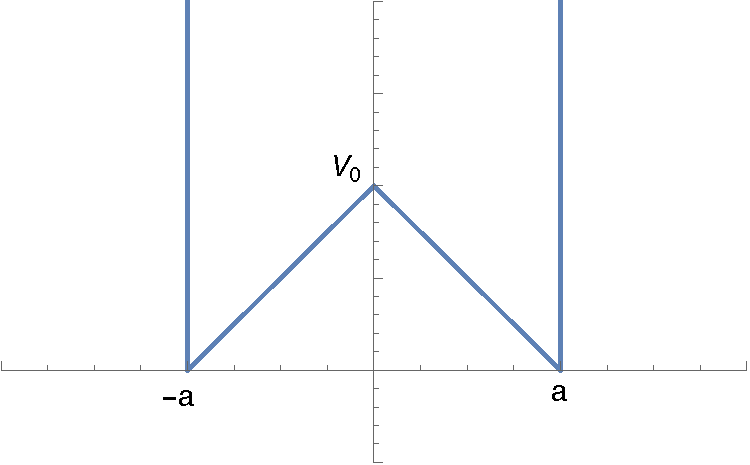
\includegraphics[width=100mm]{HW3_5a.pdf}
$$V(x)$$

\end{figure}
% 	5(b)
\item In the limit $V_0\to 0$ with $a$ fixed, what are the energy eigenvalues and eigenfunctions of the system?
\\ \\The potential in this limit is
$$\lim_{V_0\to0}V(x) = \begin{cases}0&\quad |x|<a\\\infty&\quad|x|>a\end{cases}$$
which we simply identity as the infinite square well. This is a well referenced problem, but since I have not solved it for some time, we will solve it outright. 
\\ \\To solve for the energy eigenfunctions ($\psi_E(\vect x) = \braket{\vect x|a}$ where $H\ket a  = E_a\ket a$) is to solve for the wavefunction satisfying the time-independent wave equation, namely
$$-\frac{\h^2}{2m}\nabla^2\psi_E(\vect x)+V(x)\psi_E(\vect x) = E\psi_E(\vect x).$$
Finding the eigenfunctions will amount to solving this PDE with our specified potential and boundary conditions. To begin we note that in one dimension (and dropping the energy subscript), the wave equation becomes
\begin{equation}\label{8}-\frac{\h^2}{2m}\frac{d^2\psi}{dx^2}+V(x)\psi = E\psi.\end{equation}
For $|x|>a$, $\psi = 0$, the probability of finding the particle is zero. For $|x|<a$ our potential from \eqref 7 is zero and so the wave equation is then
\begin{equation}\label{9}-\frac{\h^2}{2m}\frac{d^2\psi}{dx^2} = E\psi.\end{equation}
It is interesting to note that in order to have a normalizable wavefunction for \eqref 8, we \emph{must} have the condition that
$$E> V_{min}.$$
Confer Griffith's problem 2.2 if need be. Thus in the context of our problem, $E$ must be strictly positive. We can rewrite \eqref 9 as
$$\frac{d^2\psi}{dx^2} = -k^2$$
where
$$k\equiv \frac{\sqrt{2mE}}{\h}.$$
We should note that from the symmetry of the potential, $\psi$ can be either even or odd since the probability $|\psi|^2$ of finding the particle on either side of the origin is equivalent. Alternatively, we could show that \eqref 9 has a differential operator $\mathcal{L}(x)=\mathcal{L}(-x)$ that is even under parity which must lead us to the same conclusion, but I am unclear exactly how this works (confer Arfken 351). Typically, you start this equation off in terms of $\sin$'s and $\cos$'s and quickly implement boundary conditions to arrive at $\psi\propto\sin$ or $\psi\propto\cos$ but since I am curious to do it, I will start off with a general exponential solution. It is easy to see that the general solution (sum of two linearly independent solutions) is
$$\psi(x) = Ae^{ikx}+Be^{-ikx}.$$
Since our eigenfunction must be zero outside the square well, we match it at the boundary
$$\psi(-a) = \psi(a) = 0$$
\begin{equation}\label{10}Ae^{-ika} + Be^{ika} =0\end{equation}
\begin{equation}\label{11} Ae^{ika} +Be^{-ika} = 0.\end{equation}
If we are careful in analyzing \eqref{10} and \eqref{11} we can see that there are two possibilities:
$$ka = \frac{\pi n}{2}\quad\text{where}\quad n = 1,3,5,..$$ and
$$A=B$$
or
$$ka = \frac{\pi n}{2}\quad\text{where}\quad n = 0,2,4,..$$
and
$$A=-B.$$
Putting these into trigonometric form, we have
$$\psi_1(x) = A(e^{i\frac{\pi n}{a}x}+e^{-i\frac{\pi n}{a}x}) = C\cos\left(\frac{\pi n}{2a}x\right)\ \ \text{for}\ n=1,3,5,..$$
$$\psi_2(x) = A(e^{i\frac{\pi n}{a}x}-e^{-i\frac{\pi n}{a}x}) = D\sin\left(\frac{\pi n}{2a}x\right)\ \ \text{for}\ n=0,2,4,..$$
where we have taken the imaginary part of $\psi_2$. Thus our even and odd solutions. However, $n=0$ leads to a a trivial non-normalizable solution so we will exclude it. Lastly, we need to normalize the undetermined coefficients:
\begin{align*}C^2\int_{-a}^a{dx\ \cos^2\left(\frac{\pi n}{2a}x\right) }&= 2C^2\int_{0}^a{dx\ \left[\frac{1}{2}+\frac{\cos\left(\frac{\pi n}{a}x\right)}{2}\right]}\\
&=C^2a+C^2\frac{a}{\pi n}\left.\sin\left(\frac{\pi n}{a}x\right)\right|_0^a\\
&=C^2a+C^2\frac{a}{\pi n}\sin(\pi n)\\
1&=C^2a\\
\frac{1}{\sqrt a} &= C.
\end{align*}
For $\psi_2$ we have the same result:
\begin{align*}D^2\int_{-a}^a{dx\ \sin^2\left(\frac{\pi n}{2a}x\right) }&= D^2a-D^2\frac{a}{\pi n}\left.\sin\left(\frac{\pi n}{a}x\right)\right|_0^a\\
\frac{1}{\sqrt a}&=D.
\end{align*}
The energy eigenfunctions and energy eigenvalues of the system are
$$\psi(x) = \begin{cases} \psi_{even}(x)=\frac{1}{\sqrt a}\cos\left(\frac{\pi n}{2a}x\right)\ \ \text{for}\ n = 1,3,5,..\\
\psi_{odd}(x)\;\,= \frac{1}{\sqrt a}\sin\left(\frac{\pi n}{2a}x\right)\ \ \text{for}\ n = 2,4,6,..\end{cases}$$
$$E = \frac{n^2\pi^2\h^2}{8ma^2}.$$
% 	5(c)
\item In the limit $a\to0$ with fixed $V_0$, what are the energy eigenvalues and eigenfunctions of the system? Express the answers in terms of a small but nonzero value for $a$. 
\\ \\If we are to take our potential and do the limit
$$\lim_{a\to0}{\begin{cases}V_0\left(\frac{a-|x|}{a}\right)&\quad |x|<a\\\infty&\quad|x|>a\end{cases}}$$
we would simply wind up at a potential is everywhere infinite. Instead, a better approach might be to think about the limiting behavior as an infinite square well with a small but finite perturbation at the bottom of the well. The results of the infinite square well are 
$$\psi(x) = \begin{cases} \psi_{even}(x)=\frac{1}{\sqrt a}\cos\left(\frac{\pi n}{2a}x\right)\ \ \text{for}\ n = 1,3,5,..\\
\psi_{odd}(x)\;\,= \frac{1}{\sqrt a}\sin\left(\frac{\pi n}{2a}x\right)\ \ \text{for}\ n = 2,4,6,..\end{cases}$$
$$E = \frac{n^2\pi^2\h^2}{8ma^2}.$$ We can see that as $a\to 0$ we find that $E\to\infty$. At a nonzero value of $a$ what we will find is that 
$$E\gg V_0$$
since all the energy values are shifted up. The value of $V_0$ becomes negligible and it is as if we have an infinite square well with a very small width. If we were to expand our wave functions ($x\ll 1$ since $a\ll 1$) we find that 
$$\psi(x) = \begin{cases} \psi_{even}(x)=\frac{1}{\sqrt a}\left(1-(\frac{\pi nx}{4a})^2+..\right)\ \ \text{for}\ n = 1,3,5,..\\
\psi_{odd}(x)\;\,= \frac{1}{\sqrt a}\left(\frac{\pi nx}{2a}-\frac{\left(\frac{\pi nx}{2a}\right)^3}{6}+..\right)\ \ \text{for}\ n = 2,4,6,..\end{cases}$$
I could use only the first order terms, but I'm not sure this is the correct route to proceed. 
\\ \\\emph{Where do I go from here? How can I express $E$ and $\psi(x)$ in terms of a non-zero $a$ that differs from the infinite square well? Am I supposed to used perturbation theory here?}\\
% 	5(d)
\item What are the energy eigenvalues and eigenfunctions of the system for the general case of arbitrary $V_0$ and $a$?
 \\ \\You should label the zeros of $Ai(z)$ as $\alpha_1,\alpha_2$... and of its first derivative as $\alpha'_1$, $\alpha'_2$... in order of increasing magnitude. Likewise the zeros of $Bi(z)$ should be written as $\beta_1$, $\beta_2$... and of its first derivative as $\beta'_1$, $\beta'_2$... You may find the following properties of the Airy functions to be useful in solving this problem:
$$Ai(z) \to \frac{1}{\sqrt\pi}|z|^{-1/4}\cos(\xi-\frac{\pi}{4})\ \ \text{for}\ \  z\ll0;\quad\frac{1}{2\sqrt\pi}z^{-1/4}e^{-\xi}\ \ \text{for}\ \  z\gg0 $$
$$Bi(z) \to -\frac{1}{\sqrt\pi}|z|^{-1/4}\sin(\xi-\frac{\pi}{4})\ \ \text{for}\ \  z\ll0;\quad\frac{1}{\sqrt\pi}z^{-1/4}e^{\xi}\ \ \text{for}\ \  z\gg0 $$
$$\xi = \frac{2}{3}|z|^{3/2};\qquad z= \left[\frac{2mV_0}{\hbar^2a}\right]^{1/3}(a_0-|x|)$$
\\ \\ Let's first analyze our situation and note some conditions. 
\begin{enumerate}
\item Symmetric potential $\rightarrow\ \psi_{even}\ \text{and}\ \psi_{odd}$
\item $\psi$ is everywhere continuous
\item $\displaystyle \left.\frac{d\psi}{dx}\right|_0$ is continuous
\item BC: $\psi(-a) = \psi(a) = 0$
\item $\displaystyle \left.\frac{d\psi_{even}}{dx}\right|_0=0$
\item $\psi_{odd}(0) = 0$
\end{enumerate}
Since our solutions are even or odd, we are then allowed to solve the time-independent Schrodinger equation 
$$-\frac{\h^2}{2m}\frac{d^2\psi}{dx^2}+V(x)\psi = E\psi$$
for $x\ge0$. To gain the solutions in the negative region, we simply note that 
$$\psi(-x) = \psi(x)\quad\text{for}\quad \psi_{even}$$
and
$$\psi(-x) = -\psi(x)\quad\text{for}\quad \psi_{odd}.$$ We now begin the TISE (time-indepdenent Schrodinger equation)
$$-\frac{\h^2}{2m}\frac{d^2\psi}{dx^2}+\frac{V_0}{a}(a-x)\psi = E\psi\quad\text{for}\quad x\ge0.$$
Rearranging we have
$$-\frac{\h^2a}{2mV_0}\frac{d^2\psi}{dx^2}+(a-x)\psi = \frac{a}{V_0}E\psi$$
$$-\frac{\h^2a}{2mV_0}\frac{d^2\psi}{dx^2}+(a-\frac{a}{V_0}E-x)\psi = 0.$$
At this point, we will make a succession of substitutions that will allow us to get our equation into the appropriate Airy differential equation form. Define the dimensionless length scale ($[m^{-1}]$)
$$x_0 \equiv \frac{2mV_0}{\h^2a}^{1/3}$$
and
$$a_0 \equiv \left[a-\frac{a}{V_0}E\right]$$
to arrive at
$$-\frac{1}{x_0^3}\frac{d^2\psi}{dx^2}+(a_0-x)\psi = 0$$
$$-\frac{1}{x_0^2}\frac{d^2\psi}{dx^2}+x_0(a_0-x)\psi = 0.$$
Our final definition, the dimensionless independent variable in our Airy D.E. is 
$$z\equiv \left[\frac{2mV_0}{\h^2a}\right]^{1/3}(a_0-x)=x_0(a_0-x).$$
Since we have redefined $x$, we will need to adjust the differential operators as well. For one variable, this can be accomplished by noting the relationship of a total differential:
$$\frac{df}{dx}dx = \frac{df}{dz}dz\to\frac{df}{dx} = \frac{df}{dz}\frac{dz}{dx}\to\frac{d}{dx} = \frac{d}{dz}\frac{dz}{dx}.$$
Now applying to our present case,
$$\frac{d^2}{dx^2} = \frac{d^2}{dz^2}\left(\frac{dz}{dx}\right)^2 = \frac{d^2}{dz^2}\left[\frac{2mV_0}{\h^2a}\right]^{2/3}=x_0^2\frac{d^2}{dz^2}.$$
Substituting in, 
$$-\frac{d^2\psi}{dz^2}+x_0(a_0-x)\psi = 0 $$
$$\frac{d^2\psi}{dz^2}-z\psi = 0.$$
Alas we have arrived at our Airy differential equation. The solutions are of course the two linearly independent Airy functions. Taken as a linear superposition, our solution for $\psi(x)$ for $x\ge0$ is
$$\psi(z) = C_1Ai(z)+C_2Bi(z).$$
Our boundary condition at the infinite potential wall gives us
$$\psi(z(a)) = C_1Ai[z(a)]+C_2Bi[z(a)] = 0.$$
Once this boundary solution is satisfied, we then can construct even and odd solutions by implementing the boundary conditions. For even solutions we must have
$$\psi(z(0)) = C_1Ai[z(0)]+C_2Bi[z(0)]= 0.$$
For odd solutions we then have
$$\psi'(z(0)) = C_1Ai'[z(0)]+C_2Bi'[z(0)]= 0.$$
Without the infinite barrier, we would set one constant to zero and use the boundary condition at the origin to equate the energy to a factor proportional to one of the zero's of the Airy function, thus quantizing the energy levels. However, this is not the case here, since we have another boundary condition that must be satisfied. In total these are our conditions:
\\ \\For $\psi_{odd}$:
$$C_1Ai[z(0)]+C_2Bi[z(0)] = 0$$
$$C_1Ai[z(a)]+C_2Bi[z(a)] = 0$$
For $\psi_{even}$:
$$C_1Ai'[z(0)]+C_2Bi'[z(0)]= 0$$
$$C_1Ai[z(a)]+C_2Bi[z(a)] = 0$$
As homogeneous linear equations, solutions only exist if the determinant is zero.
\\ \\$\psi_{odd}:$
$$\begin{vmatrix}Ai[z(0)]&Bi[z(0)]\\Ai[z(a)]&Bi[z(a)]
\end{vmatrix}=0$$
\\$\psi_{even}:$
$$\begin{vmatrix}Ai'[z(0)]&Bi'[z(0)]\\Ai[z(a)]&Bi[z(a)]
\end{vmatrix}=0$$
These determinants can most likely be equated to zero and we expect many solutions to exist for the following reason: for $E\gg V_0$, our situation is nearly that of the infinite square well, which we know has an infinite number of energy eigenvalues. 
\\ \\
Perhaps an alternative approach here, would be to solve the system using only the energy. We start with the full form of our points of interest for our odd wavefunctions:
$$z(0) = x_0a\left(-\frac{E}{V_0}+1\right)$$
$$z(a) = x_0a\left(-\frac{E}{V_0}\right).$$
Firstly, we know that $E>V_{min}$ and thus $E>0$. Therefore, we see that $z(0)>z(a)$. Now, the first zero of either $Ai(z)$ or $Bi(z)$ must occur at $z<0$. For an appropriate value of $E$, we can see that if the zeros of the Airy functions differed by $x_0a$, then our condition would be satisfied for a single energy. Working with the Airy functions of the first kind, we can impose the condition
$$\alpha_i = x_0a\left(-\frac{E}{V_0}\right)$$
or
$$E = -\frac{V_0}{x_0a}\alpha_i.$$
The criteria on the second zero is then
$$\alpha_j = x_0a+\alpha_i.$$
We could numerically cycle through all the zeros of the Airy function and for those with a separation of
$$\alpha_j-\alpha_i=x_0a$$
we would then have a corresponding energy of
$$E = -\frac{V_0}{x_0a}\alpha_i.$$
Applying the same concept to both even and odd wavefucntions we have:
$$\psi_{even}(z) = C_1Ai(z);\quad E = -\frac{V_0}{x_0a}\alpha_i;\quad\alpha'_j -\alpha_i= x_0a$$
$$\psi_{odd}(z) = C_2Ai(z);\quad E = -\frac{V_0}{x_0a}\alpha_i;\quad\alpha_j -\alpha_i= x_0a$$
$$\psi_{even}(z) = C_3Bi(z);\quad E = -\frac{V_0}{x_0a}\beta_i;\quad\beta'_j -\beta_i= x_0a$$
$$\psi_{odd}(z) = C_4Bi(z);\quad E = -\frac{V_0}{x_0a}\beta_i;\quad\beta_j -\beta_i= x_0a$$
where the third column denotes the condition that must be satisfied by our zeros, $C_i$ is the appropriate normalization constant for each wavefunction, and
$$z\equiv \left[\frac{2mV_0}{\h^2a}\right]^{1/3}(a_0-x)=x_0(a_0-x);\quad a_0 \equiv \left[a-\frac{a}{V_0}E\right].$$
In looking at a graph of the Airy function, we can see that at $z\ll 0$ the ``wavelength'' is very small and so there should be a great number of possible zero's that will satisfy our criteria. In the same light, at this range of $z$, our energies will be very large and we have the semblance of the infinite square well. 

\end{enumerate}
% #6
\item
A particle of mass $m$ moving in one dimension is confined to a space $0<x<L$ by an infinite well potential. In addition the particle experiences a delta function potential of strength $\lambda >0$, given by $\lambda\delta(x-L/2)$ located at the center of the well. Find a trancendental equation for the energy eigenvalues $E$ in terms of the mass $m$, the potential strength $\lambda$, and the size of the well $L$. 
\\ \\ As always, we start by solving the TISE for $\psi$ for a given potential. For $0<x<L/2$ we have zero potential and thus we have 
$$\psi_-(x) = Ae^{-ikx}+Be^{ikx}$$
while for $L/2<x<L$ we have
$$\psi_-(x) = Ce^{-ikx}+De^{ikx}$$
where 
$$k\equiv\frac{\sqrt{2mE}}{\h}$$
and we note that $E>0$.
For the left side we impose the boundary condition
$$\psi_-(0) = A+B=0$$
$$A=-B$$ in which our wavefunction becomes (absorbing an $i$ into the coeffcient)
$$\psi_-(x) = A\sin(kx).$$
For the right hand side we have
$$\psi_+(L) = Ce^{-ikL}+De^{ikL}=0.$$
If we are clever, we could set
$$C = e^{ikL};\quad D=-e^{-ikL}$$
which would satisfy the potential at the end of the well and give us a wavefunction of
$$\psi_+(x) = C\sin(kx-kL) = C\sin(k(L-x))$$
where I have been keeping the same constant while absorbing things. 
Continuity at the middle of well requires
$$\psi_-(L/2) = \psi_+(L/2)$$
$$A\sin(k\frac{L}{2}) = C\sin(k\frac{L}{2})$$
and thus 
$$A=C.$$
Therefore we now have a wavefunction of
$$\psi(x) = \begin{cases}A\sin(kx)&\quad\text{for}\quad 0<x<L/2\\A\sin(k(L-x))&\quad\text{for}\quad L/2<x<L\end{cases}.$$ 
Our last condition, which is to find the discontinuity at $x=L/2$ will impose the conditions on our energies. Borrowing from problem 3 we have
$$\Delta\left(\frac{d\psi}{dx}\right)= \frac{2m}{\h^2}\lim_{\epsilon\to L/2}\int_{-\epsilon}^{+\epsilon}{dx\ V(x)\psi(x)}
$$
$$-Ak\cos\left(k\frac{L}{2}\right)-Ak\cos\left(k\frac{L}{2}\right)= \frac{2m}{\h^2}\lim_{\epsilon\to L/2}\int_{-\epsilon}^{+\epsilon}{dx\ \lambda\delta(x-L/2)\psi(x)}$$
$$-2Ak\cos\left(k\frac{L}{2}\right)= \frac{2m\lambda}{\h^2}A\sin\left(k\frac{L}{2}\right)$$
$$k = -\frac{m\lambda}{\h^2}\tan\left(k\frac{L}{2}\right).$$
In terms of energy we then have
$$\frac{\sqrt{2mE}}{\h} = -\frac{m\lambda}{\h^2}\tan\left(\frac{\sqrt{2mE}L}{2\h}\right)$$
$$E = \frac{m\lambda^2}{2\h^2}\tan^2\left(\frac{\sqrt{2mE}L}{2\h}\right).$$

% #7
\item
Consider the potential
$$V(x) = -\frac{\h^2a^2}{m}\sech^2(ax)$$
where $a$ is a positive constant.
\begin{enumerate}
% 	7(a)
\item
Show that potential has a bound state $\psi_0(x) = A\sech(ax)$. Calculate the energy of the state.
\begin{figure}[H]
\centering
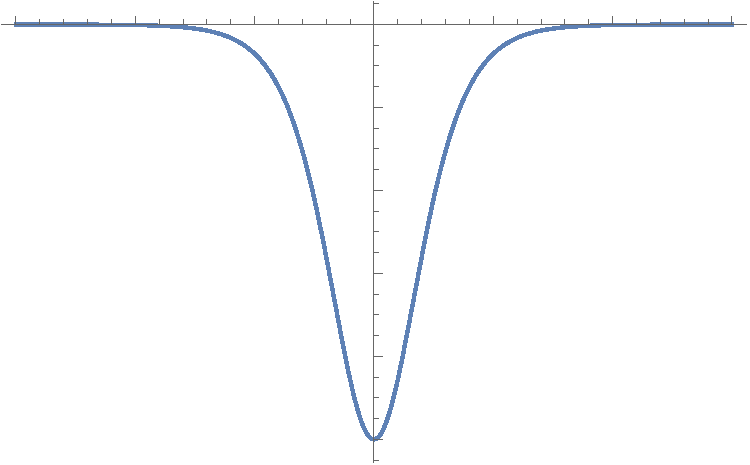
\includegraphics[width=100mm]{HW3_7a.pdf}
$$f(x) = -\sech^2(ax)$$
\end{figure}
To show that it has a bound state ($E<0$) and find the energy we will substitute it into the TISE. First note that
\begin{align*}\frac{d}{dx^2}[\sech(ax)]  &= \frac{d}{dx}[-a\sech(ax)\tanh(ax)]\\
&=a^2\sech(ax)\tanh^2(ax)-a^2\sech(ax)\sech^2(ax)\\
&=a^2\sech(ax)\tanh^2(ax)-a^2\sech^3(ax).
\end{align*}
For the TISE we once again have
$$-\frac{\h^2}{2m}\frac{d^2\psi}{dx^2}+V(x)\psi = E\psi.$$
Now using
$$\psi_0(x) = A\sech(ax),$$ we form
$$-\frac{\hbar^2}{2m}A[a^2\sech(ax)\tanh^2(ax)-a^2\sech^3(ax)]-\frac{\h^2a^2}{m}\sech^2(ax)[A\sech(ax)] = E[A\sech(ax)] $$
$$-\frac{\hbar^2a^2}{m}A[\sech(ax)\tanh^2(ax)-\sech^3(ax)]+\frac{\h^2a^2}{m}(\tanh^2(ax)-1)[2A\sech(ax)] = E[2A\sech(ax)] $$
$$\frac{\h^2a^2}{m}A\sech(ax)\tanh^2(ax)+\frac{\h^2a^2}{m}A\sech^3(ax)-\frac{\h^2A^2}{m}2a\sech(ax) = E[2a\sech(ax)]$$
$$\frac{\h^2a^2}{m}\tanh^2(ax)+\frac{\h^2a^2}{m}\sech^2(ax)-\frac{\h^2a^2}{m}2 = 2E$$
$$\frac{\h^2a^2}{m}-\frac{\h^2a^2}{m}2 = 2E$$
$$E = -\frac{\h^2a^2}{2m}$$
\begin{figure}[H]
\centering
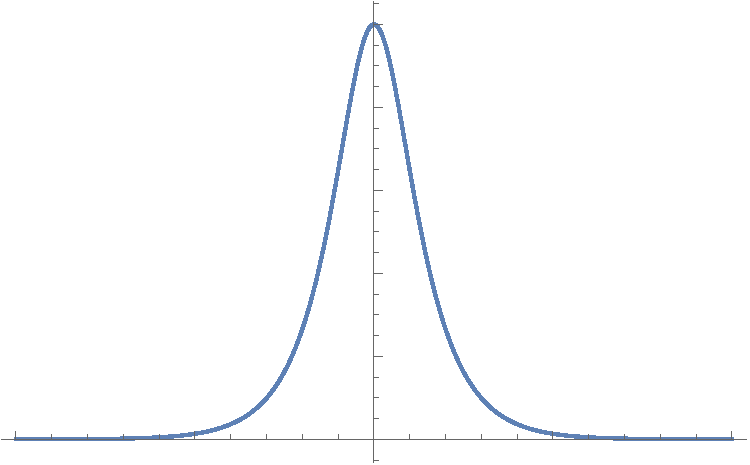
\includegraphics[width=100mm]{HW3_7a1.pdf}
$$f(x) = \sech(ax)$$
\end{figure}

% 	7(b)
\item
Use the WKB approximation to estimate this energy and compare with the exact result. 
\\ \\In the WKB approximation, we approximate our wavefunction as
$$\psi(x) \cong \frac{A}{\sqrt{p(x)}}e^{\frac{i}{\h}\int{dx\  p(x)}}+\frac{B}{\sqrt{p(x)}}e^{-\frac{i}{\h}\int{dx\  p(x)}}$$
where $$p(x) \equiv \sqrt{2m[E-V(x)]}.$$
Within the potential well, $E>V(x)$ and so $p(x)$ is real. Outside the well $E<V(x)$ and thus $p(x)$ is imaginary. Lets label our two turning points as $x_1$ and $x_2$ where $x_1$ is negative (left hand turning point) and $x_2$ is positive (right hand turning point). Consequently, our potential can be divided into three regions and $\psi$ will go as
$$\psi(x) = \begin{cases} \displaystyle\frac{C_1}{\sqrt{|p(x)|}}e^{\frac{1}{\h}\int_x^{x_1}{dx\  |p(x)|}}+\frac{C_2}{\sqrt{|p(x)|}}e^{-\frac{1}{\h}\int_x^{x_1}{dx\  |p(x)|}}&\quad\text{for}\quad x<x_1\\ \\
 \displaystyle\frac{C_3}{\sqrt{p(x)}}e^{\frac{i}{\h}\int_{x_1}^{x_2}{dx\  p(x)}}+\frac{C_4}{\sqrt{p(x)}}e^{-\frac{i}{\h}\int_{x_1}^{x_2}{dx\  p(x)}}&\quad\text{for}\quad x_1<x<x_2\\ \\
  \displaystyle\frac{C_5}{\sqrt{|p(x)|}}e^{\frac{1}{\h}\int{dx\  |p(x)|}}+\frac{C_6}{\sqrt{|p(x)|}}e^{-\frac{1}{\h}\int{dx\  |p(x)|}}&\quad\text{for}\quad x>x_2
\end{cases}
$$
Notice that the wave functions for regions I and III have $E<V(x)$, hence the exponential behavior. For region I, we note that as $x\to\infty$ the first exponential blows up, thus $C_1 = 0$. Similarly, for region III $C_5 = 0$. In factoring out $i$ in the integral from region I and III, note that we must use $|p(x)|$ if we are to use its same definition. Otherwise, we will need to redesignate it as $p(x) = \sqrt{2m(V(x)-E)}$. Additionally, we can absorb an $i$ into the constant terms for the factor in front. In connecting the various regions, it is advisable to shift the origin of the region of interest such that the turning point occurs at $x_1$ or $x_2$. Otherwise, the resulting integrals give some unwieldy functions to work with. It is a simple matter to change the turning point to its original form afterward. Thus from herein forth we assume the turning points lie at the origin. 
\\ \\To connect region I to region II, we approximate the potential at the turning point to be
$$V(x) \cong V(0)+V'(0)x = E+V'(0)x.$$
It is very important to note that here $V'(0)$ is negative. For this linear potential we must, of course, have the Airy functions as solutions:
$$-\frac{\h^2}{2m}\frac{d^2\psi}{dx^2}+[E-|V'(0)|x]\psi = E\psi$$
$$\frac{d^2\psi}{dx^2} = -\alpha^3x\psi$$
where
$$\alpha \equiv \left[\frac{2m}{\h^2}|V'(0)|\right]^{1/3}.$$
Now define 
$$z\equiv -\alpha x$$
so
$$\frac{d^2\psi}{dz^2} = z\psi$$
and thus
$$\psi_A(x) = c_1Ai(-\alpha x)+c_2Bi(-\alpha x).$$
This is the wavefunction in the neighborhood of the turning point $x_1$. In this overlap region,
\begin{equation}\label{p1}p(x) = \sqrt{2m(E-V(x))} = \sqrt{2m(E-E+|V'(0)|x)} = \h\alpha^{3/2}\sqrt{x}.\end{equation}
In region I we have the WKB wavefunction
$$\psi_I(x) =\frac{C_2}{\sqrt{|p(x)|}}e^{-\frac{1}{\h}\int_x^{0}{dx\  |p(x)|}}$$
with the integral
$$\int_x^{0}{dx\ |p(x)|} = \hbar\alpha^{3/2}\int_x^{0}{dx\ x^{1/2}} = \frac{2}{3}\h(-\alpha x)^{3/2}$$
and thus the wavefunction in region I is 
$$\psi_1(x) = \frac{C_2}{\sqrt\h\alpha^{3/4}(-x)^{1/4}}e^{-\frac{2}{3}(-\alpha x)^{3/2}}.$$
We need to connect this to our Airy function. We will actually use the asymptotic form of the Airy function for this region. Why? Firstly, I'm not sure how else we could connect it, since the Airy function is not in a closed form and we want to avoid numerical work here. Secondly, it turns out that approximating the Airy function in its asymptotic form is accurate (up to a very reasonable degree of error, which we could quantify if we chose to) as long as the range of which the potential can still be approximated to first order is long enough for $Ai(z)$ to approach asymptotic behavior. In fact, this criteria is not as stringent as it sounds (cf. Griffiths problem 8.8). For $x<0$ note that we have $z>0$, thus we need the asymptotic form of the Airy function for $z\gg0$:
$$\psi_A(x) = \frac{c_1}{2\sqrt\pi (-\alpha x)^{1/4}}e^{-\frac{2}{3}(-\alpha x)^{3/2}}+\frac{c_2}{\sqrt\pi (-\alpha x)^{1/4}}e^{\frac{2}{3}(-\alpha x)^{3/2}}.$$
Comparing $\psi_A(x)$ to $\psi_I(x)$ we see that
 $$c_2 = 0$$ 
 \begin{equation}\label{c_1}c_1 = 2C_2\sqrt{\frac{\pi}{\alpha\h}}.\end{equation}
 Now connecting region II, we start with the WKB wavefunction:
 $$\psi_{2}(x) = \frac{C_3}{\sqrt{p(x)}}e^{\frac{i}{\h}\int_{0}^x{dx\  p(x)}}+\frac{C_4}{\sqrt{p(x)}}e^{-\frac{i}{\h}\int_{0}^x{dx\  p(x)}}.$$
Although in region II $E<V$, $p(x)$ remains the same as in \eqref{p1} so
$$\int_0^{x}{dx\ p(x)} = \hbar\alpha^{3/2}\int_0^{x}{dx\ x^{1/2}} = \frac{2}{3}\h(\alpha x)^{3/2}$$
and our new WKB wavefunction is
 $$\psi_{2}(x) = \frac{C_3}{\sqrt\h\alpha^{3/4}x^{1/4}}e^{i\frac{2}{3}(\alpha x)^{3/2}}+\frac{C_4}{\sqrt\h\alpha^{3/4}x^{1/4}}e^{-i\frac{2}{3}(\alpha x)^{3/2}}.$$
 Keeping in mind that we set $b=0$ earlier and that $z\equiv(-\alpha x)$, we note that the asymptotic form of the Airy function for $x>0$ yields $z<0$ and thus we use $z\ll 0$ as the asymptotic form:
 \begin{align*}\psi_A(x) &= \frac{c_1}{\sqrt\pi(\alpha x)^{1/4}}\sin\left[\frac{2}{3}(\alpha x)^{3/2}+\frac{\pi}{4}\right]\\
 &=\frac{c_1}{\sqrt\pi(\alpha x)^{1/4}}\frac{1}{2i}\left[e^{i\frac{\pi}{4}}e^{i\frac{2}{3}(\alpha x)^{3/2}}-e^{-i\frac{\pi}{4}}e^{-i\frac{2}{3}(\alpha x)^{3/2}}\right].
 \end{align*}
 In comparison of of $\psi_A(x)$ to $\psi_2(x)$ we see that
 $$C_3 = \frac{c_1}{2i}\sqrt{\frac{\alpha\h}{\pi}}e^{i\frac{\pi}{4}}$$
 $$C_4 = -\frac{c_1}{2i}\sqrt{\frac{\alpha\h}{\pi}}e^{-i\frac{\pi}{4}}.$$
 Now we can insert the result from \eqref{c_1} to arrive at
  $$C_3 = -ie^{i\frac{\pi}{4}}C_2$$
  $$C_4 = ie^{-i\frac{\pi}{4}}C_2.$$
 We have successfully connected region I to region II - all we needed was to find the coefficient connections. Both outside and inside the neighborhood of the turning point, our regional wave functions are now
$$\psi_1(x) = \frac{C_2}{\sqrt{|p(x)|}}e^{-\frac{1}{\h}\int_x^0{dx\ |p(x)|}}$$
 \begin{align*}\psi_{2}(x) &= -\frac{iC_2}{\sqrt{p(x)}}\left[e^{\frac{i}{\h}\int^x_0{dx\ p(x)}+i\frac{\pi}{4}}-e^{-\frac{i}{\h}\int^x_0{dx\ p(x)}-i\frac{\pi}{4}}\right]\\
 &=\frac{2C_2}{\sqrt{p(x)}}\sin\left[\frac{1}{\h}\int_0^x{dx\ p(x)}+\frac{\pi}{4}\right].\end{align*}
 Shifting the origin back to the turning point $x_1$, we now have
 $$\psi(x) = \begin{cases} \displaystyle\frac{C_2}{\sqrt{|p(x)|}}e^{-\frac{1}{\h}\int_x^{x_1}{dx\ |p(x)|}}&\quad\text{for}\quad x<x_1\\ \\\displaystyle
\frac{2C_2}{\sqrt{p(x)}}\sin\left[\frac{1}{\h}\int_{x_1}^x{dx\ p(x)}+\frac{\pi}{4}\right]&\quad\text{for}\quad x_1<x \end{cases}$$
 Our next task amounts to finding the connection formulas for turning point $x_2$. One might think to start with the wavefunction already found for region II, however it will be nicely general to repeat our same procedure for the $x_2$ turning point and connect them afterward. This allows us to find the connection formulas for any potential configuration in the future. We start with the general wavefunction in region II with the origin shifted to the turning point:
 $$\psi_2(x) = \frac{C_3}{\sqrt{p(x)}}e^{\frac{i}{\h}\int^{0}_x{dx\  p(x)}}+\frac{C_4}{\sqrt{p(x)}}e^{-\frac{i}{\h}\int_{x}^{0}{dx\  p(x)}}$$
 approximate the potential in the neighborhood of $x_2$ to be
 $$V(x) \cong  E+V'(0)x,$$
 solve the Schrodinger equation (no absolute value signs of $V'(0)$ since we have a positive slope this time)
 $$-\frac{\h^2}{2m}\frac{d^2\psi}{dx^2}+[E+V'(0)x]\psi = E\psi$$
$$\frac{d^2\psi}{dx^2} = \alpha^3x\psi$$
where
$$\alpha \equiv \left[\frac{2m}{\h^2}V'(0)\right]^{1/3}.$$
and
$$z\equiv \alpha x$$
so
$$\frac{d^2\psi}{dz^2} = z\psi$$
and thus
$$\psi_A(x) = c_1Ai(\alpha x)+c_2Bi(\alpha x).$$
We now find the $p(x)$ we need:
$$p(x) = \sqrt{2m(E-V(x))} = \sqrt{2m(E-E-V'(0)x)} = \h\alpha^{3/2}\sqrt{-x}.$$
For region II we integrate
$$\int_x^{0}{dx\ p(x)} = \hbar\alpha^{3/2}\int_x^{0}{dx\ (-x)^{1/2}} = \frac{2}{3}\h(-\alpha x)^{3/2}$$
and $\psi_2(x)$ becomes
 $$\psi_{2}(x) = \frac{C_3}{\sqrt\h\alpha^{3/4}(-x)^{1/4}}e^{i\frac{2}{3}(-\alpha x)^{3/2}}+\frac{C_4}{\sqrt\h\alpha^{3/4}(-x)^{1/4}}e^{-i\frac{2}{3}(-\alpha x)^{3/2}}.$$
With the turning point at the origin, region II corresponds to $x<0$ and so the correct asymptotic form of the Airy function is $z\ll 0$
 \begin{align*}\psi_A(x) &= \frac{c_1}{\sqrt\pi(-\alpha x)^{1/4}}\sin\left[\frac{2}{3}(-\alpha x)^{3/2}+\frac{\pi}{4}\right]\\
 &=\frac{c_1}{\sqrt\pi(-\alpha x)^{1/4}}\frac{1}{2i}\left[e^{i\frac{\pi}{4}}e^{i\frac{2}{3}(-\alpha x)^{3/2}}-e^{-i\frac{\pi}{4}}e^{-i\frac{2}{3}(-\alpha x)^{3/2}}\right].
 \end{align*}
 In comparing $\psi_A(x)$ to $\psi_2(x)$
 we see that 
 $$C_3 = \frac{c_1}{2i}\sqrt{\frac{\alpha\h}{\pi}}e^{i\frac{\pi}{4}}$$
 $$C_4 = -\frac{c_1}{2i}\sqrt{\frac{\alpha\h}{\pi}}e^{-i\frac{\pi}{4}}.$$
 Now forging onward to region III, which has a wavefunction given by
 $$\psi_3(x) =  \frac{C_6}{\sqrt{|p(x)|}}e^{-\frac{1}{\h}\int{dx\  |p(x)|}}$$
 we note that
 $$|p(x)| = \h\alpha^{3/2}\sqrt{x}$$
 and so 
 $$\int_0^{x}{dx\ |p(x)|} = \hbar\alpha^{3/2}\int_0^{x}{dx\ x^{1/2}} = \frac{2}{3}\h(\alpha x)^{3/2}.$$
 Thus the wavefunction now becomes
$$\psi_3(x) = \frac{C_6}{\sqrt\h\alpha^{3/4}x^{1/4}}e^{-\frac{2}{3}(\alpha x)^{3/2}}.$$
In this region $(x>0)$ and so our asymptotic Airy function is $z\gg 0$
$$\psi_A(x) = \frac{c_1}{2\sqrt\pi (\alpha x)^{1/4}}e^{-\frac{2}{3}(\alpha x)^{3/2}}+\frac{c_2}{\sqrt\pi (\alpha x)^{1/4}}e^{\frac{2}{3}(\alpha x)^{3/2}}.$$
 In comparing $\psi_A(x)$ to $\psi_3(x)$ we see that
$$c_1 = 2C_6\sqrt{\frac{\pi}{\alpha\h}}$$
   $$c_2 = 0.$$ 
   Now we can substitute this $c_2$ into our coefficients $C_3$ and $C_4$ found earlier to arrive at
   $$C_3 = -ie^{i\frac{\pi}{4}}C_6$$
   $$C_4 = ie^{-i\frac{\pi}{4}}C_6.$$
   We have successfully connected region II to region III.  Both outside and inside the neighborhood of the turning point, our regional wave functions are now
 \begin{align*}\psi_{2}(x) &= -\frac{iC_6}{\sqrt{p(x)}}\left[e^{\frac{i}{\h}\int^0_x{dx\ p(x)}+i\frac{\pi}{4}}-e^{-\frac{i}{\h}\int^0_x{dx\ p(x)}-i\frac{\pi}{4}}\right]\\
 &=\frac{2C_6}{\sqrt{p(x)}}\sin\left[\frac{1}{\h}\int_x^0{dx\ p(x)}+\frac{\pi}{4}\right].\end{align*}
 $$\psi_3(x) = \frac{C_6}{\sqrt{|p(x)|}}e^{-\frac{1}{\h}\int_0^x{dx\ |p(x)|}}.$$
 Shifting the origin back, the wavefunction in all regions can now be expressed in total as
  $$\psi(x) \cong \begin{cases} \displaystyle\frac{C_2}{\sqrt{|p(x)|}}e^{-\frac{1}{\h}\int_x^{x_1}{dx\ |p(x)|}}&\quad\text{for}\quad x<x_1\\ \\\displaystyle
\frac{2C_2}{\sqrt{p(x)}}\sin\left[\frac{1}{\h}\int_{x_1}^x{dx\ p(x)}+\frac{\pi}{4}\right]&\quad\text{for}\quad x_1<x\\ \\\displaystyle
\frac{2C_6}{\sqrt{p(x)}}\sin\left[\frac{1}{\h}\int_x^{x_2}{dx\ p(x)}+\frac{\pi}{4}\right]&\quad\text{for}\quad x<x_2
\\ \\\displaystyle
 \frac{C_6}{\sqrt{|p(x)|}}e^{-\frac{1}{\h}\int_{x_2}^x{dx\  |p(x)|}}&\quad\text{for}\quad x>x_2.
 \end{cases}$$
 These are our connection formulas. The first two represent a connection for a negative slope and the last two for a positive slope. They can be utilized to approximate any potential as long as it satisfies our WKB criteria ($\lambda\ll\frac{E-V(x)}{|dV/dx|}$ cf. Sakura 2.5.60). For our problem all that remains is to equate the two wave functions in region II together. The coefficients are easily handled and it is then necessary that the arguments of the sine functions must be equivalent. Denoting
 $$\theta_1(x) = -\frac{1}{\h}\int_{x_1}^x{dx\ p(x)}-\frac{\pi}{4}$$
 $$\theta_2(x) = \frac{1}{\h}\int_{x}^{x_2}{dx\ p(x)}+\frac{\pi}{4}$$
we have
 $$\theta_1(x)+n\pi = \theta_2(x)\quad\text{for}\quad n = 0,1,2,3..$$
 since  the relative minus can be absorbed into either coefficient. Thus
$$-\frac{1}{\h}\int_{x_1}^x{dx\ p(x)}-\frac{\pi}{4}+n\pi= \frac{1}{\h}\int_{x}^{x_2}{dx\ p(x)}+\frac{\pi}{4}$$
\begin{equation}\label{quant}\int_{x_1}^{x_2}{dx\ p(x)} = \left(n-\frac{1}{2}\right)\pi\h\quad\text{for}\quad n=1,2,3..\end{equation}
This is our quantization condition for the allowed energies! Why was $n=0$ not included? Well this would imply 
$$\int_{x_1}^{x_2}{dx\ p(x)} = \int_{x_1}^{x_2}{dx\ \sqrt{2m(E-V(x))}} = -\frac{\pi}{2}\h.$$
For $E$ to be real, we must have $p(x)>0$ and the integral of a strictly positive integrand over increasing bounds must itself be positive. Thus we cannot have negative values of the action integral if we are to have a real energy. For any bound state with nonsingular $V'(x)$ at the turning points, we can simply use \eqref{quant} to find the energies. 
\\ \\For our problem at hand, this amounts to using 
$$V(x) = -\frac{\h^2a^2}{m}\sech^2(ax)$$
in
$$\int_{x_1}^{x_2}{dx \sqrt{2m(E-V(x))}} = \int_{x_1}^{x_2}{dx \sqrt{2m(E+\frac{\h^2a^2}{m}\sech^2(ax))}} = \left(n-\frac{1}{2}\right)\pi\h.$$
Note that the potential is an even function. Therefore we have
$$2\int_0^{x_2}{dx \sqrt{2m(E+\frac{\h^2a^2}{m}\sech^2(ax))}}  =2\sqrt2\hbar a\int_0^{x_2}{dx\ \sqrt{\sech^2(ax)+\frac{mE}{\h^2a^2}}}. $$
For our integration limit, we have
$$E=V(x_2)$$
$$E = -\frac{\h^2a^2}{m}\sech^2{ax_2}.$$
To make things simpler, lets denote
$$b\equiv -\frac{mE}{\h^2a^2};\quad z\equiv\sech^2(ax),$$
therefore 
$$x=\frac{1}{a}\sech^{-1}\sqrt z$$
$$dx = \frac{1}{a}\left(\frac{-1}{\sqrt z\sqrt{(1-z)}}\right)\frac{1}{\sqrt 2z}dz=-\frac{1}{2a}\frac{1}{z\sqrt{(1-z)}}dz .$$
Before we make these substitutions into our integral, lets compute our integration limits:
$$0\to\sech^2(0) = 1;\quad x_2\to\sech^2(ax_2) = -\frac{mE}{\h^2a^2} = b.$$
Now we have the integral
$$2\sqrt2\h a\left(-\frac{1}{2a}\right)\int_1^b{\frac{\sqrt{z-b}}{z\sqrt{1-z}}dz}  = \sqrt 2\h\int_b^1{\frac{1}{z}\sqrt{\frac{z-b}{1-z}}dz}.$$
We can split up the integrand into two separate fractions and rationalize the denominator
$$\frac{1}{z}\sqrt{\frac{z-b}{1-z}} = \frac{1}{\sqrt{(1-z)(z-b)}}-\frac{b}{z\sqrt{(1-z)(z-b)}}.$$
Now integrating these things
\begin{align*}\sqrt2 \h\int_b^1{dz\ \frac{1}{\sqrt{(1-z)(z-b)}}} &= \sqrt2\h\left.\left[-2\tan^{-1}\sqrt{\frac{1-z}{z-b}}\right]\right|_b^1\\
&=\sqrt2\h\left[-2\tan^{-1}(0)+2\tan^{-1}(\infty)\right] \\
&= \sqrt 2\pi
\end{align*}
\begin{align*}\-\sqrt 2\h b\int_b^1{dz\ \frac{1}{z\sqrt{-b+(1+b)z-z^2}}} &= -\h\sqrt b\sin^{-1}\left.\left[\frac{(1+b)z-2b}{z(1-b)}\right]\right|_b^1\\
&=\sqrt 2\h\left[-\sqrt b\sin^{-1}(1)+\sqrt b\sin^{-1}(-1)\right]\\
&=\sqrt 2\h(-\sqrt b\frac{\pi}{2}-\sqrt b\frac{\pi}{2})\\
&=-\sqrt 2\h\sqrt b\pi.
\end{align*}
Adding together we have
$$\sqrt 2 \h\pi(1-\sqrt b) = \left(n-\frac{1}{2}\right)\pi\h$$
$$1-\sqrt b=\frac{n-\frac{1}{2}}{\sqrt 2}$$
$$\sqrt b = 1-\frac{1}{\sqrt 2}\left(n-\frac{1}{2}\right)$$
$$\left(-\frac{mE}{\h^2a^2}\right)^{1/2} = 1-\frac{1}{\sqrt 2}\left(n-\frac{1}{2}\right).$$
Since we have a bound state $E<0$ here and we can write this as
$$\left(\frac{m|E|}{\h^2a^2}\right)^{1/2} = 1-\frac{1}{\sqrt 2}\left(n-\frac{1}{2}\right).$$
Since the LHS is strictly positive, we must then have
$$\left(n-\frac{1}{2}\right)<\sqrt 2$$
$$n<\sqrt 2+\frac{1}{2}.$$
Under this condition we must then have 
$$n=1$$
in which
$$\left(-\frac{mE}{\h^2a^2}\right)^{1/2} = 1-\frac{1}{\sqrt 2}\left(\frac{1}{2}\right)= 1-\frac{\sqrt 2}{4} = \frac{4-\sqrt{2}}{4}$$
$$E=-\frac{\h^2a^2}{m}\left(\frac{4-\sqrt 2}{4}\right)^2$$
$$E=-\frac{\h^2a^2}{m}\left(\frac{4-\sqrt 2}{4}\right)^2.$$
Numerically, this equates to
$$E = -\frac{\h^2a^2}{m}(.418)$$
while our exact result from part (a) yielded
$$E = -\frac{\h^2a^2}{2m}.$$
A decent approximation indeed.
\end{enumerate}
\end{enumerate}
\end{document}
